\documentclass[serif, xcolor=dvipsnames]{beamer}

\makeatletter

% HAY QUE ELEGIR EL QUE CORRESPONDA

% \usepackage{mathpazo}%Letra palatino con fuentes para matemáticas
\usepackage[T1]{fontenc}
\usepackage[utf8]{inputenc}
\usepackage{graphicx}
\usepackage{url}
\usepackage{amsmath}
\usepackage{booktabs}
\usepackage{textcomp}%%needed for the euro symbol

\date{}

\usepackage[emulate=units]{siunitx}
\sisetup{per=fraction, fraction=nice, decimalsymbol=comma}
\newunit{\wattpeak}{Wp}
\newunit{\watthour}{Wh}
\newunit{\amperehour}{Ah}

\setbeamercovered{transparent}
\setbeamertemplate{navigation symbols}{}
\usefonttheme{structuresmallcapsserif} 
\usefonttheme{serif} 
\usefonttheme{structurebold}

%\usepackage{epstopdf}


\usepackage[spanish]{babel}
\addto\shorthandsspanish{\spanishdeactivate{~<>}}

\hypersetup{pdfauthor={Oscar Perpi\~n\'an},%
    pdftitle={Energ\'ia Solar Fotovoltaica},%
    filecolor=blue,%
    urlcolor=blue}



%\usepackage{handoutWithNotes} %para hacer papel con notas 
%\pgfpagesuselayout{4 on 1 with notes}[a4paper,border shrink=5mm]



%\usepackage{pgfpages}
%\pgfpagesuselayout{2 on 1}[a4paper,border shrink=5mm]

 
% \usepackage{mathpazo}%Letra palatino con fuentes para matemáticas
\usepackage[T1]{fontenc}
\usepackage[utf8]{inputenc}
\usepackage{graphicx}
\usepackage{url}
\usepackage{amsmath}
\usepackage{booktabs}

\usepackage[spanish]{babel}
\addto\shorthandsspanish{\spanishdeactivate{~<>}}


\usepackage{hyperref}
% \hypersetup{pdfauthor={Oscar Perpi\~n\'an},%
%     pdftitle={Energ\'ia Solar Fotovoltaica},%
%     filecolor=blue,%
%     urlcolor=blue}

\hypersetup{
    bookmarks=true,         % show bookmarks bar?
%    unicode=true,          % non-Latin characters in Acrobat’s bookmarks
    bookmarksnumbered=false,
    bookmarksopen=false,
    breaklinks=true,
    backref=true,
    pdftoolbar=true,        % show Acrobat’s toolbar?
    pdfmenubar=true,        % show Acrobat’s menu?
    pdffitwindow=false,     % window fit to page when opened
    pdfstartview={FitH},    % fits the width of the page to the window
    pdftitle={Energía Solar Fotovoltaica},    % title
    pdfauthor={Oscar Perpiñán Lamigueiro},     % author
    pdfsubject={Electrotecnia},   % subject of the document
    pdfcreator={AucTeX/Emacs},   % creator of the document
    pdfproducer={LaTeX}, % producer of the document
    pdfnewwindow=true,      % links in new window
    pdfborder={0 0 0},
    colorlinks=true,       % false: boxed links; true: colored links
    linkcolor=,          % color of internal links
    citecolor=BrickRed,        % color of links to bibliography
    filecolor=black,      % color of file links
    urlcolor=Blue           % color of external links 
}

\usepackage[emulate=units]{siunitx}
\sisetup{per=fraction, fraction=nice, decimalsymbol=comma}
\newunit{\wattpeak}{Wp}
\newunit{\watthour}{Wh}
\newunit{\amperehour}{Ah}

\setbeamercovered{transparent}
\setbeamertemplate{navigation symbols}{}
\usefonttheme{serif} 
\usefonttheme{structuresmallcapsserif} 

\useinnertheme[shadow=true]{rounded}
\useoutertheme{shadow}
%\usecolortheme[named=BrickRed]{structure} %sirve para cambiar el color genérico
\usecolortheme{orchid}
\usecolortheme{whale}
\documentclass[xcolor={usenames,svgnames,dvipsnames}]{beamer}
\usepackage[utf8]{inputenc}
\usepackage[T1]{fontenc}
\usepackage{graphicx}
\usepackage{grffile}
\usepackage{longtable}
\usepackage{wrapfig}
\usepackage{rotating}
\usepackage[normalem]{ulem}
\usepackage{amsmath}
\usepackage{textcomp}
\usepackage{amssymb}
\usepackage{capt-of}
\usepackage{hyperref}
\usepackage{color}
\usepackage{listings}
\usepackage{mathpazo}
\usepackage{gensymb}
\usepackage{amsmath}
\usepackage{chemarr}%flechas para reacciones químicas (SFER.tex)
\bibliographystyle{plain}
\AtBeginSubsection[]{\begin{frame}[plain]\tableofcontents[currentsubsection,sectionstyle=show/shaded,subsectionstyle=show/shaded/hide]\end{frame}}
\AtBeginSection[]{\begin{frame}[plain]\tableofcontents[currentsection,hideallsubsections]\end{frame}}
\usepackage[emulate=units]{siunitx}
\sisetup{fraction=nice, decimalsymbol=comma, retain-unity-mantissa = false}
\newunit{\wattpeak}{Wp}
\newunit{\watthour}{Wh}
\newunit{\amperehour}{Ah}
\usepackage{steinmetz}
\hypersetup{colorlinks=true, linkcolor=OliveGreen, urlcolor=Blue}
\renewcommand{\thefootnote}{\fnsymbol{footnote}}
\beamertemplatenavigationsymbolsempty
\setbeamertemplate{footline}[frame number]

\setbeamercolor{alerted text}{fg=Green!50!black} \setbeamerfont{alerted text}{series=\bfseries}
\usefonttheme{serif}
\setbeamercovered{transparent}
\setbeamertemplate{navigation symbols}{}
\usefonttheme{serif} 

\setbeamercolor{palette primary}{bg=OliveGreen,fg=white}
\setbeamercolor{palette secondary}{bg=OliveGreen,fg=white}
\setbeamercolor{palette tertiary}{bg=OliveGreen,fg=white}
\setbeamercolor{palette quaternary}{bg=OliveGreen,fg=white}
\setbeamercolor{structure}{fg=OliveGreen} % itemize, enumerate, etc
\setbeamercolor{section in toc}{fg=OliveGreen} % TOC sections

\usetheme[hideothersubsections]{Goettingen}

\usepackage{tikz}

\titlegraphic{
\includegraphics[width=2.5cm]{../figs/logoEOI.jpg}}
\addtobeamertemplate{frametitle}{}{%
\begin{tikzpicture}[remember picture,overlay]
\node[anchor=south east,yshift=2pt] at (current page.south east) {
\includegraphics[width=1.5cm]{../figs/logoEOI.jpg}};
\end{tikzpicture}}


\makeatother

\usepackage[spanish]{babel}
\addto\shorthandsspanish{\spanishdeactivate{~<>}}

\begin{document}

\title[\textsc{SFCR: Conceptos Generales}]{\textsc{Sistemas Fotovoltaicos }\\
  \textsc{de Conexión a Red}}


\subtitle{Conceptos Generales}


\author{\textsc{Oscar Perpiñán Lamigueiro}} \date{}

\frame[plain]{\titlepage}

\AtBeginSection[]{
  \begin{frame}[plain]
    \frametitle{Índice}
    % \setcounter{tocdepth}{1}
    \tableofcontents[currentsection]
  \end{frame}

} \selectlanguage{spanish}%

\section{Conceptos Generales}


\begin{frame}
  \frametitle{Definición de un SFCR}

  \begin{block}{}
    Un Sistema Fotovoltaico Conectado a la Red (SFCR) es un sistema
    cuya función es producir energía eléctrica en condiciones
    adecuadas para poder ser inyectada en la red convencional.
  \end{block}

  \begin{center}
    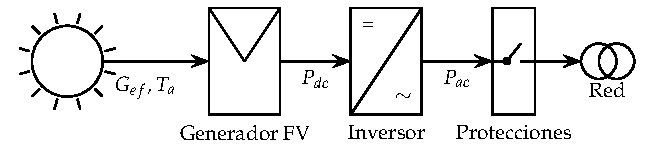
\includegraphics{../Figuras/EsquemaSFCR}
    \par\end{center}
\end{frame}

\begin{frame}
  \frametitle{Mecanismos de retribución}

  \begin{block}{}
    La energía producida por este sistema será consumida parcial o
    totalmente en las cercanías, y la energía sobrante será inyectada
    en la red para su distribución a otros puntos de consumo.
  \end{block}

  \begin{block}{Mecanismos de retribución}
    \begin{itemize}
    \item Prima (\emph{Feed-in tariff})
    \item Balance neto (\emph{Net-metering})
    \end{itemize}
  \end{block}

\end{frame}

\begin{frame}
  \frametitle{Retribución con prima}
  \begin{itemize}
  \item Ingresos por la energía total producida (independientemente de
    la que haya sido consumida en las cercanías del SFCR).
  \item El diseño no necesita considerar un consumo a satisfacer.
  \item Objetivo: producción anual del sistema sea la máxima posible
    sin tomar en consideración los consumos cercanos.
  \end{itemize}
\end{frame}

\begin{frame}
  \frametitle{Balance neto}
  \begin{itemize}
  \item Compensa los saldos de energía eléctrica entre el SFCR y un
    sistema de consumo asociado.
  \item Cuando la producción del SFCR supera al consumo, la red
    eléctrica absorbe el excedente puntual, generándose derechos de
    consumo diferido.
  \item Estos derechos de consumo se pueden ejercer cuando la
    producción del SFCR no es suficiente para satisfacer el consumo
    asociado.
  \item El diseño debe incluir el consumo asociado como una variable
    adicional que condicionará el tamaño del generador fotovoltaico.

  \end{itemize}
\end{frame}

% \begin{frame}
%   \frametitle{Normativa aplicable en España}
%   \begin{itemize}

%   \item RD. 1578/2008 / RD 661/2007 /RD 436/2004:
%     \begin{itemize}
%     \item Marcan primas por la venta de la energía producida
%     \item Procedimiento administrativo de legalización
%     \item Dos tipos de SFCR (Edificios y Terreno) con variedad de
%       primas.
%     \item Sistema de cupos.
%     \end{itemize}

%   \item RD. 1565/2010
%     \begin{itemize}
%     \item Modifica al 1578/2008 y 661/2007.
%     \item Reduce primas.
%     \end{itemize}

%   \end{itemize}
% \end{frame}

% \begin{frame}
%   \frametitle{Normativa aplicable en España}
%   \begin{itemize}

%   \item RD. 1699/2011
%     \begin{itemize}
%     \item Establece las condiciones administrativas, contractuales,
%       económicas y técnicas básicas para la conexión a las redes de
%       distribución de energía eléctrica de las instalaciones
%       fotovoltaicas (además de otras tecnologías) de potencia no
%       superior a $\SI{100}{\kilo\watt}$.
%     \item Describe los requisitos técnicos de conexión a red que un
%       SFCR debe cumplir, dedicando especial atención a los sistemas de
%       seguridad eléctrica.
%     \item Simplifica las tramitaciones para la conexión de pequeñas
%       instalaciones de generación eléctrica.
%     \item Posibilidad de conexión en la red interior de un consumidor.
%     \item Fija el contrato-tipo que debe ser firmado por el usuario
%       del SFCR y la compañía eléctrica a la que se conecta el sistema.
%     \item Deroga el RD. 1663/2000 y modifica algunos aspectos del
%       RD. 1578/2008.
%     \end{itemize}


%   \end{itemize}

% \end{frame}

% \begin{frame}
%   \frametitle{Normativa aplicable en España}
%   \begin{itemize}
%   \item Reglamento Electrotécnico de Baja Tensión (no hay un capítulo
%     específico)
%   \item Documento HE5 del Codigo Técnico de la Edificación
%   \end{itemize}

% \end{frame}

\begin{frame}
  \frametitle{Características distintivas sobre suelo y en
    edificación}
  \begin{itemize}
  \item \textbf{Sobre suelo}

    \begin{itemize}
    \item Sistemas estáticos, con una inclinación y orientación fija
    \item Sistemas de seguimiento, que varían la posición del
      generador a lo largo del día y año para maximizar la radiación
      efectiva incidente
    \end{itemize}
  \item \textbf{Sobre edificación}, según el grado de integración

    \begin{itemize}
    \item General
    \item Superposición de módulos: colocación paralela a la
      envolvente del edificio
    \item Integración arquitectónica: doble función energética y
      arquitectónica; sustituyen elementos constructivos
      convencionales o son elementos constituyentes de la composición
      arquitectónica
    \end{itemize}
  \end{itemize}

\end{frame}
\begin{frame}
  \frametitle{SFCR sobre suelo}
  \begin{itemize}
  \item \textbf{Objetivo}: maximizar la producción energética anual
    del sistema con el menor coste y la menor ocupación de terreno
    posibles
  \item El diseñador debe decidir el tamaño del generador teniendo en
    cuenta:

    \begin{itemize}
    \item Inversión económica (relacionada principalmente con la
      potencia del generador)
    \item Rendimiento económico deseado (relacionado con la energía
      producida por el sistema y, por tanto, con el modo de
      seguimiento empleado)
    \item Ocupación de terreno (relacionado con el modo de seguimiento
      empleado).
    \end{itemize}
  \end{itemize}

\end{frame}
\begin{frame}[plain]
  \frametitle{Estructuras sobre suelo}

  \begin{center}
    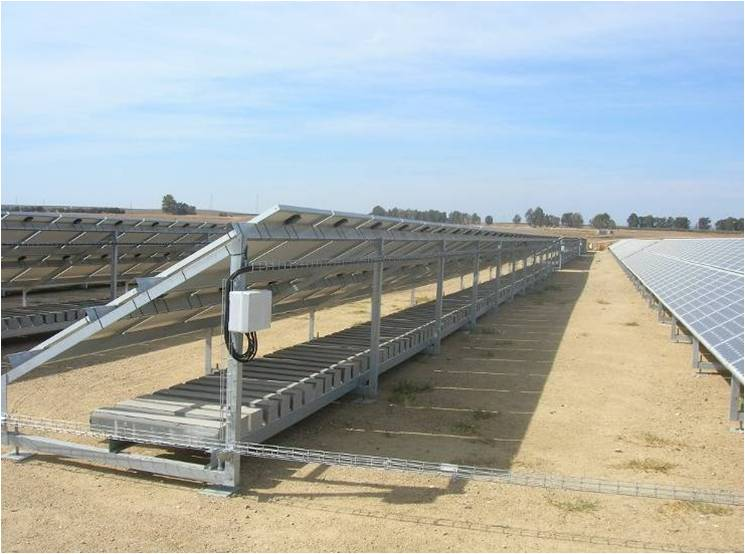
\includegraphics[scale=0.35]{../Fotos/EstructuraEstaticaSuelo}
    \par\end{center}


\end{frame}
\begin{frame}
  \frametitle{SFCR sobre suelo: seguimiento}
  \begin{itemize}
  \item \textbf{Fundamento:}

    \begin{itemize}
    \item Radiación incidente aumenta al seguir al sol
    \item Pérdidas por reflexión disminuyen si el apuntamiento al sol
      mejora
    \end{itemize}
  \item Las diferentes técnicas de seguimiento son un compromiso entre
    un apuntamiento perfecto y sistemas estructurales más económicos y
    mejores aprovechamientos del terreno.
  \end{itemize}

\end{frame}
\begin{frame}
  \frametitle{SFCR sobre suelo: seguimiento}
  \begin{itemize}
  \item \textbf{Doble eje}

    \begin{itemize}
    \item Apuntamiento {}``perfecto''
    \item Mejor productividad, peor ocupación de terreno.
    \end{itemize}
  \item \textbf{Seguimento acimutal}

    \begin{itemize}
    \item Sacrifica un movimiento (inclinación del generador) para
      conseguir sistemas más económicos.
    \end{itemize}
  \item \textbf{Seguimiento horizontal con eje Norte-Sur}

    \begin{itemize}
    \item Sencillez y estabilidad estructural (el eje es horizontal y
      paralelo al terreno, con tantos puntos de apoyo como se
      consideren necesarios),
    \item Facilidad de motorización,
    \item Buen aprovechamiento del terreno.
    \end{itemize}
  \end{itemize}

\end{frame}
\begin{frame}[plain]
  \frametitle{Seguidor de eje horizontal N-S}

  \begin{center}
    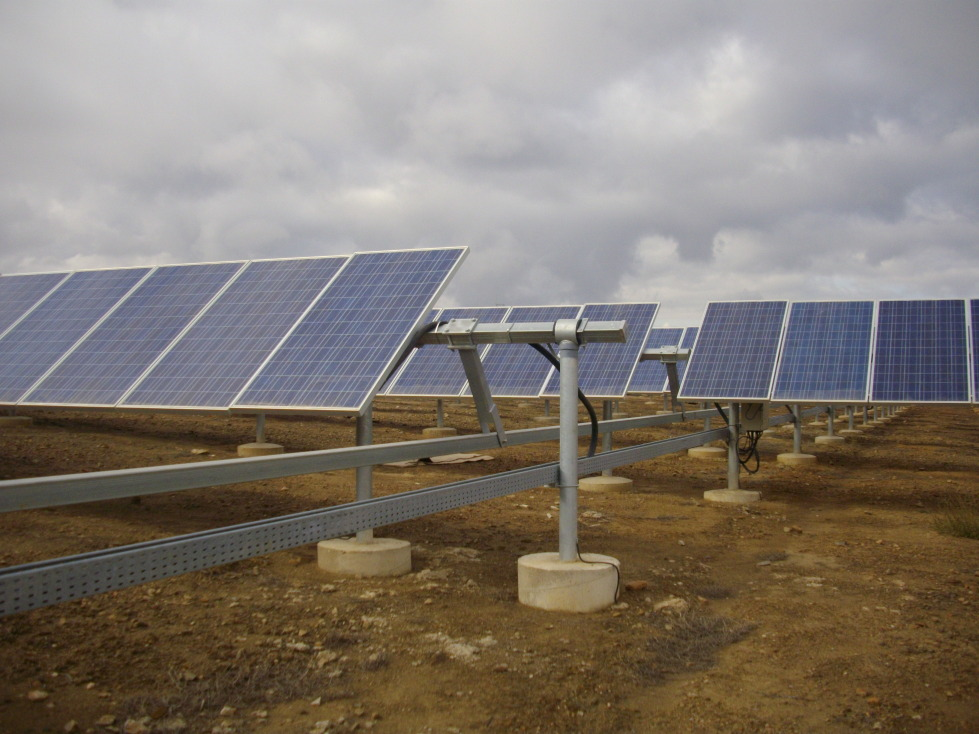
\includegraphics[scale=0.25]{../Fotos/SeguidorEjeHorizontal}
    \par\end{center}


\end{frame}
\begin{frame}[plain]
  \frametitle{Seguidor de doble eje}

  \begin{center}
    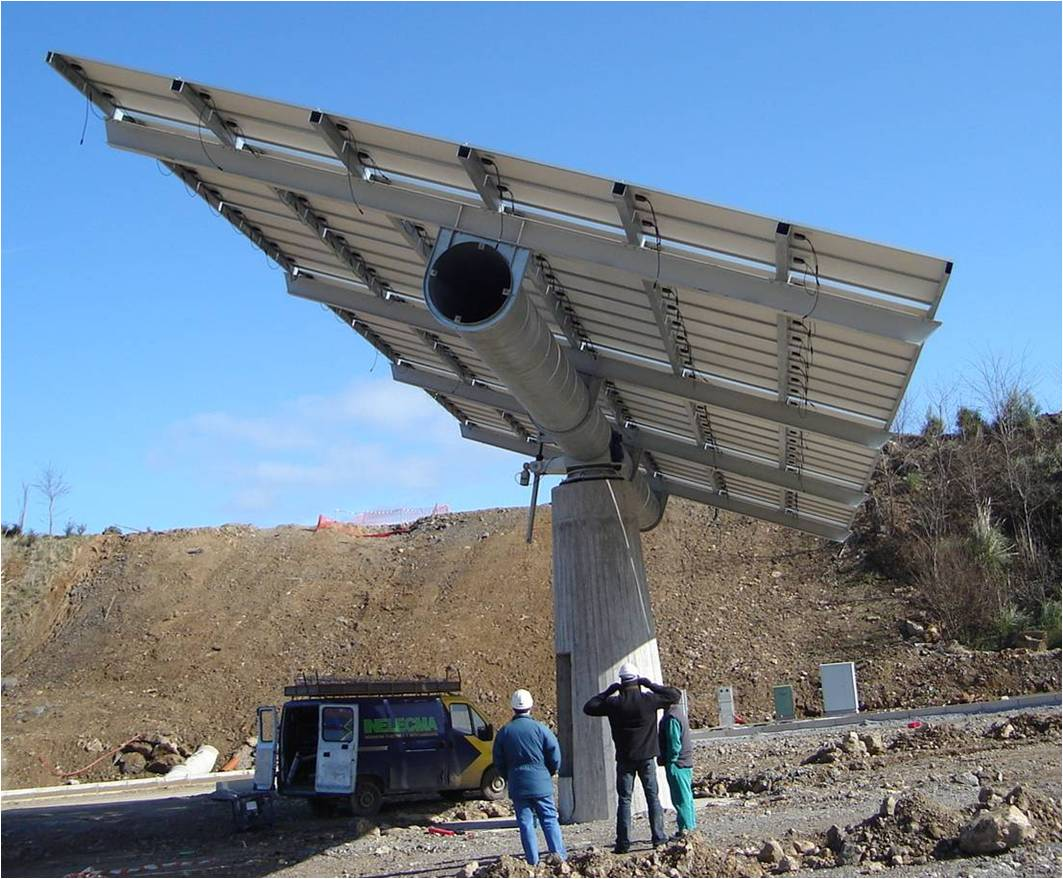
\includegraphics[scale=0.4]{../Fotos/SeguidorReocin}
    \par\end{center}


\end{frame}
\begin{frame}
  \frametitle{SFCR en edificación}
  \begin{block} {}

    La integración del sistema fotovoltaico con el edificio exige
    tener en cuenta muchos factores que condicionan la ubicación y la
    configuración del generador.

    El diseñador debe tomar las decisiones oportunas para
    \textbf{aprovechar las sinergias entre edificio y sistema
      fotovoltaico}, reduciendo las posibles interferencias entre uno
    y otro.

  \end{block}
  \begin{center}
    \url{http://www.pvdatabase.org/}
    \par\end{center}


\end{frame}
\begin{frame}
  \frametitle{Integración arquitectónica}
  \begin{columns}[c]%{}


    \column{6cm}

    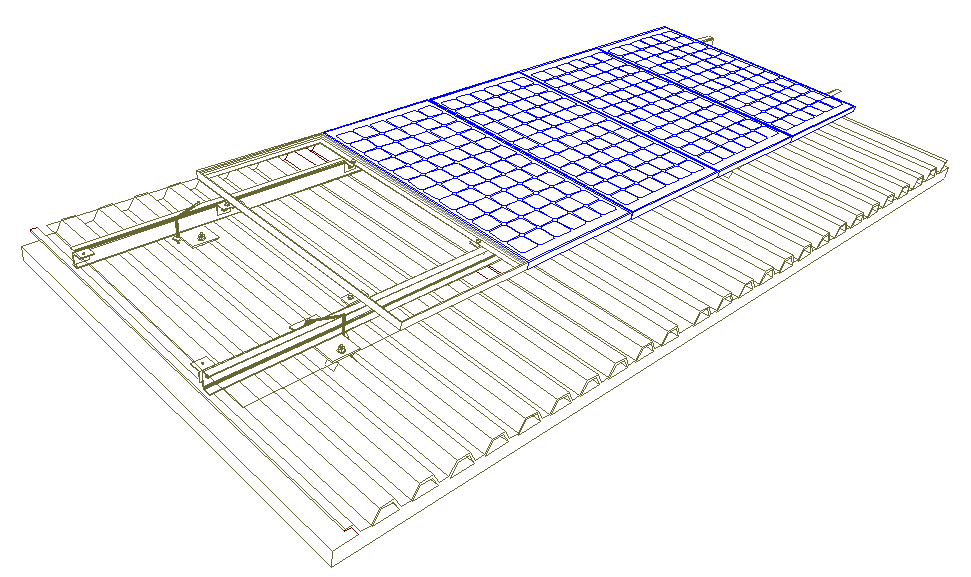
\includegraphics[scale=0.35]{../Figuras/Figuras_Externas/CubiertaInclinada}


    \column{4cm}

    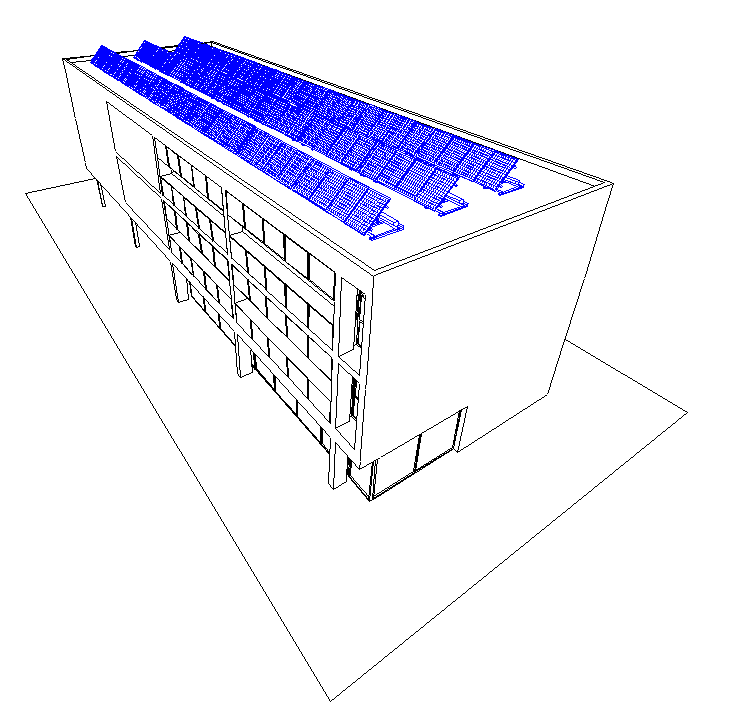
\includegraphics[scale=0.35]{../Figuras/Figuras_Externas/CubiertaPlana}

  \end{columns}%{}

\end{frame}
\begin{frame}
  \frametitle{Integración arquitectónica}
  \begin{columns}[c]%{}


    \column{6cm}

    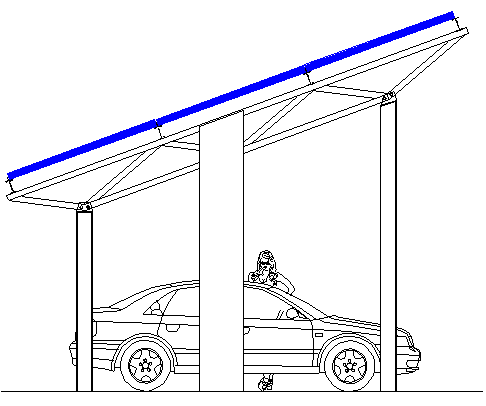
\includegraphics[scale=0.4]{../Figuras/Figuras_Externas/Aparcamiento}


    \column{4cm}

    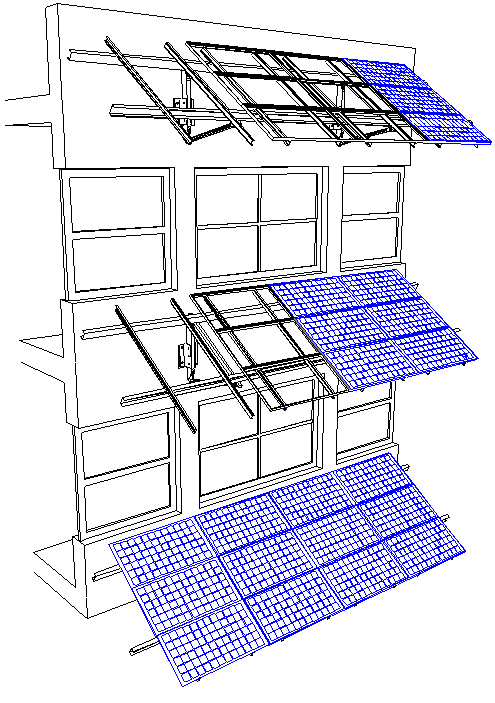
\includegraphics[scale=0.4]{../Figuras/Figuras_Externas/Parasol}

  \end{columns}%{}

\end{frame}
\begin{frame}
  \frametitle{Integración arquitectónica}
  \begin{columns}[c]%{}


    \column{6cm}

    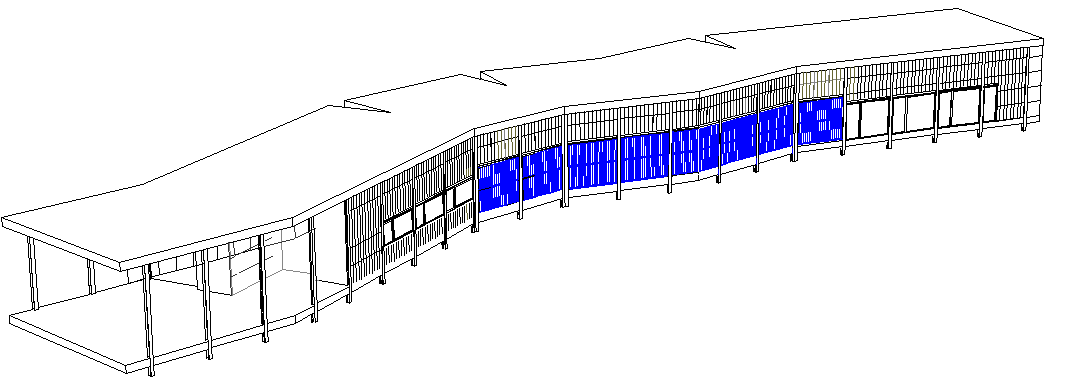
\includegraphics[scale=0.35]{../Figuras/Figuras_Externas/FachadaAcristalada}


    \column{4cm}

    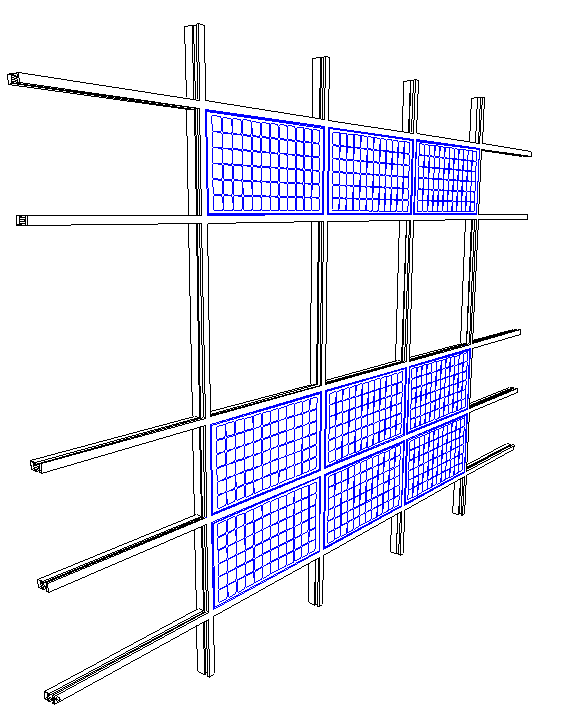
\includegraphics[scale=0.35]{../Figuras/Figuras_Externas/MuroCortina}

  \end{columns}%{}

\end{frame}

\begin{frame}
  \frametitle{SFCR en edificación: CTE-HE5}
  \begin{block} {Zonas climáticas}

    Este documento divide España en cinco zonas climáticas de acuerdo
    al valor medio anual de la radiación global diaria en el plano
    horizontal.

    Por ejemplo, toda la cornisa cantábrica está encuadrada en la zona
    I (radiación inferior a $\SI{3.8}{\kWh\per\meter\squared}$)
    mientras que Canarias y parte de Andalucía pertenecen a la zona V
    (radiación superior a $\SI{5}{\kWh\per\meter\squared}$) .

    Este Código aboga por instalar mayor potencia en las zonas con
    mayor radiación.

  \end{block}

\end{frame}
\begin{frame}
  \frametitle{SFCR en edificación: CTE}
  \begin{block} {Potencia \textbf{nominal} a instalar}

\[
P_{min}=C\cdot(0.002\cdot S - 5)\]

\begin{itemize}
\item Esta potencia debe ser superior a $\SI{5}{\kilo\watt}$ e
  inferior a $\SI{100}{\kilo\watt}$.
\item $C=1$ para zona climática I, $C=1.4$ para zona climática V.
\item Aplica sólo cuando $S > \SI{5000}{\meter\squared}$.
\end{itemize}


\end{block}

\end{frame}
\begin{frame}
  \frametitle{SFCR en edificación}
  \begin{block} {Sistemas Eléctricos}

    En este tipo de SFCR el diseño de los sistemas eléctricos debe
    tener en cuenta las canalizaciones previstas o existentes en el
    edificio.  Por facilidad de instalación y mantenimiento, y por
    seguridad de los sistemas, es recomendable el uso de
    canalizaciones separadas del resto de sistemas del edificio.

    Sin embargo, los criterios de seguridad eléctrica aconsejan
    utilizar una \textbf{red de tierras común} para el edificio y el
    sistema fotovoltaico.

  \end{block}

\end{frame}
\begin{frame}
  \frametitle{Condiciones técnicas de la conexión}
  \begin{itemize}
  \item El propietario de un generador fotovoltaico puede vender a una
    compañia eléctrica toda la energía que produce su sistema, no sólo
    la que le \textquotedblleft{}sobra\textquotedblright{} (diferencia
    entre la producción de su sistema y el consumo de, por ejemplo, su
    domicilio).
  \item La reglamentación eléctrica española establece la separación
    administrativa entre la comercialización y la distribución de la
    energía (así, la empresa que nos vende energía eléctrica en
    nuestro hogar es distinta a la que compra la energía que produce
    el sistema que podamos tener en nuestro tejado).
  \end{itemize}

\end{frame}
\begin{frame}
  \frametitle{Condiciones técnicas de la conexión}
  \begin{itemize}
  \item Por tanto, al menos administrativamente, la generación
    fotovoltaica y el consumo
    \textquotedblleft{}cercano\textquotedblright{} son dos elementos
    independientes.
  \item No obstante, es claro que la corriente eléctrica no entiende
    de leyes ni contratos, sino que fluye según las leyes de
    Kirchhoff.
  \item Así, la energía producida por un SFCR será consumida parcial o
    totalmente en el propio edificio (generación distribuida).
  \end{itemize}

\end{frame}
\begin{frame}
  \frametitle{Condiciones técnicas de la conexión}
  \begin{itemize}
  \item La separación existente entre empresa comercializadora y
    empresa distribuidora se refleja en la separación de contratos y
    facturas, y por tanto, también de elementos y puntos de medida.
  \item Es decir, no pueden utilizarse las lecturas de dos contadores
    distintos (uno de venta y otro de compra) para componer una única
    factura.
  \item Este hecho, unido a la necesidad legal de conectar el sistema
    fotovoltaico en un punto propiedad de la compañía eléctrica (por
    tanto, externo a las instalaciones eléctricas propias del
    domicilio, empresa, etc) tiene como consecuencia que en ciertos
    casos la legalización de un sistema fotovoltaico sea
    extremadamente complicada.
  \end{itemize}

\end{frame}
\begin{frame}
  \frametitle{Condiciones técnicas de la conexión}
  \begin{itemize}
  \item \textbf{Titulares con contrato de suministro en Media Tensión
      con instalaciones fotovoltaicas de potencia menor a 100 kW. }

    \begin{itemize}
    \item A pesar de que la potencia fotovoltaica es menor que el
      valor que obliga a la conexión en MT, la otra obligación de
      conexión en punto propiedad de la compañía eléctrica implica el
      uso de un transformador BT-MT distinto al usado para consumo.
    \item Sin embargo, esta solución conlleva pérdidas energéticas e
      incremento de inversión de la instalación que la pueden hacer
      inviable.
    \item La posibilidad de inyectar \textquotedblleft{}aguas
      abajo\textquotedblright{} del transformador de consumo y hacer
      los balances necesarios en las facturas de venta y consumo,
      utilizando las medidas de los respectivos contadores es posible
      bajo el RD 1699/2011.

    \end{itemize}
  \end{itemize}

\end{frame}

\begin{frame}
  \frametitle{Condiciones técnicas de la conexión}
  \begin{itemize}
  \item \textbf{Titulares en edificios de varias viviendas. }

    \begin{itemize}
    \item De nuevo, la necesidad de realizar la conexión
      \textquotedblleft{}aguas arriba\textquotedblright{} al contador
      de consumo, implica en este caso la instalación de cableado
      bajante desde la vivienda en cuestión hasta la sala de
      protecciones del edificio.
    \item Esta solución no es siempre fácil ni técnicamente (no
      siempre existe espacio o canalizaciones disponibles en la
      bajante del edificio) ni administrativamente (es necesario el
      permiso de la comunidad de vecinos).
    \end{itemize}
  \end{itemize}

\end{frame}
\section{Inversor de CR}


\begin{frame}
  \frametitle{Conceptos generales}
  \begin{block} {}

    La potencia suministrada por un generador fotovoltaico iluminado
    es de tensión continua, que debe ser adecuadamente acondicionada
    para permitir el funcionamiento correcto de las cargas conectadas
    en un sistema autónomo o el acoplamiento a la red eléctrica en el
    caso de sistemas de conexión a red.

  \end{block}

\end{frame}
\begin{frame}
  \frametitle{Conceptos generales}
  \begin{block} {}
    \begin{itemize}
    \item El equipo de acondicionamiento de potencia, denominado
      inversor DC/AC, realiza la conversión de continua a alterna
      cumpliendo con determinados requisitos de tensión eficaz,
      frecuencia, distorsión armónica de las ondas de tensión y
      corriente, rendimiento instantáneo y medio, seguridad eléctrica,
      etc.
    \item Funciona como fuente de corriente autoconmutada y
      sincronizada con la red.
    \end{itemize}
  \end{block}

\end{frame}
\begin{frame}
  \frametitle{Tipos de inversores}

  A grandes rasgos, los inversores pueden agruparse en tres
  categorías:
  \begin{itemize}
  \item \textbf{Inversor central}: un único inversor dedicado a todo
    el generador (o a un conjunto de ramas)
  \item \textbf{Inversor orientado a rama} (\emph{string-inverter}):
    un inversor dedicado a una rama del generador.
  \item \textbf{{}``Módulo-AC}'': un inversor dedicado a un módulo del
    generador.
  \end{itemize}

\end{frame}
\begin{frame}
  \frametitle{Tipos de inversores}
  \begin{itemize}
  \item Los \textbf{inversores orientados a rama} son particularmente
    útiles en algunos sistemas de integración arquitectónica, al poder
    adaptarse mejor a las condiciones de funcionamiento con
    orientaciones e inclinaciones diversas.
  \item Los inversores
    \textbf{\textquotedblleft{}módulo-AC\textquotedblright{}} deben
    descartarse en cualquier caso (salvo pequeños sistemas
    demostrativos).
  \end{itemize}

\end{frame}
\begin{frame}
  \frametitle{Tipos de inversores}
  \begin{itemize}
  \item Los \textbf{inversores centrales} son recomendables para
    instalaciones de medio o gran tamaño. Permiten reducir costes (de
    adquisición, instalación y mantenimiento) y aumentar fiabilidad y
    eficiencia.
  \item \textbf{La potencia del inversor debe estar en consonancia con
      la potencia del generador} (una planta de 1 MWp debiera contar
    con 10 inversores de 100 kW o 4 de 250 kW, pero no con 200 de 5
    kW).
  \end{itemize}

\end{frame}
\begin{frame}
  \frametitle{Características de un inversor comercial}
  \begin{itemize}
  \item \textbf{Potencia nominal y máxima}, siendo ésta un porcentaje
    de sobrecarga que el equipo es capaz de soportar durante un
    determinado período de tiempo (indicado por el fabricante).
  \item \textbf{Ventana de búsqueda del Punto de Máxima Potencia} (MPP
    en siglas inglesas): es el rango de tensiones en las que el
    inversor aplica un algoritmo de búsqueda del MPP del generador
    fotovoltaico.
  \end{itemize}

\end{frame}
\begin{frame}
  \frametitle{Características de un inversor comercial}
  \begin{itemize}
  \item \textbf{Tensión máxima de entrada}: es la máxima tensión que
    el inversor puede aguantar sin sufrir una avería.
  \item \textbf{Tensión nominal de salida}: es la tensión de red a la
    que se puede conectar el inversor (habitualmente 230 Vac para
    equipos monofásicos y 400 Vac para equipos trifásicos).
  \item \textbf{Umbral de arranque}: según las unidades en las que se
    expresa, puede indicar la radiación solar incidente en el
    generador ($\si{\watt\per\meter\squared}$) o la potencia de
    entrada (W) necesaria para que el inversor comience el proceso de
    conversión.
  \end{itemize}

\end{frame}
\begin{frame}
  \frametitle{Características de un inversor comercial}
  \begin{itemize}
  \item \textbf{Eficiencia máxima}: máximo valor que toma la relación
    entre potencia de salida y potencia de entrada. En inversores de
    calidad la eficiencia es estable en un amplio rango de
    funcionamiento del equipo y de un valor cercano a la eficiencia
    máxima.
  \item \textbf{Rendimiento europeo}: es la relación entre la energía
    entregada por un inversor que recibe una energía producida por un
    generador fotovoltaico funcionando en unas condiciones de
    radiación características de la zona centroeuropea.
  \end{itemize}

\end{frame}
\begin{frame}[plain]
  \frametitle{Composición}

  \begin{center}
    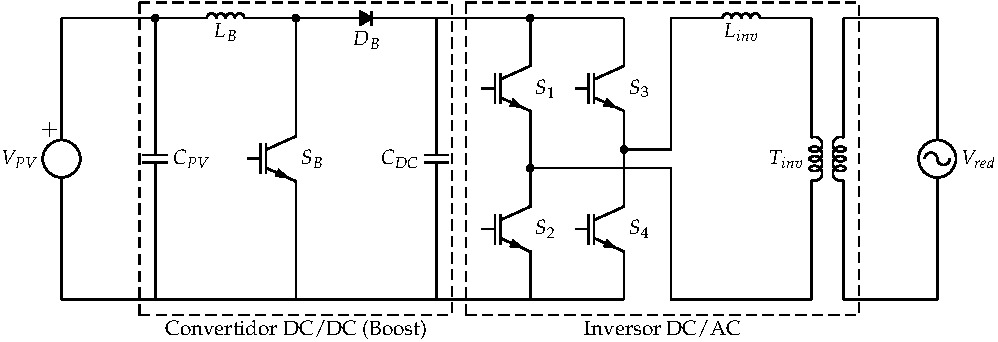
\includegraphics[scale=0.6]{../Figuras/InversorPV}
    \par\end{center}
  \begin{itemize}
  \item \textbf{Filtro de entrada}: atenúa el rizado que produce la
    conmutación en la corriente de entrada
  \item \textbf{Convertidor DC/DC}: adecúa (eleva o reduce) la tensión
    de salida del generador a la tensión necesaria para el puente de
    conmutación.  Puede realizar las funciones de búsqueda del punto
    de máxima potencia.
  \end{itemize}

\end{frame}
\begin{frame}[plain]
  \frametitle{Composición}

  \begin{center}
    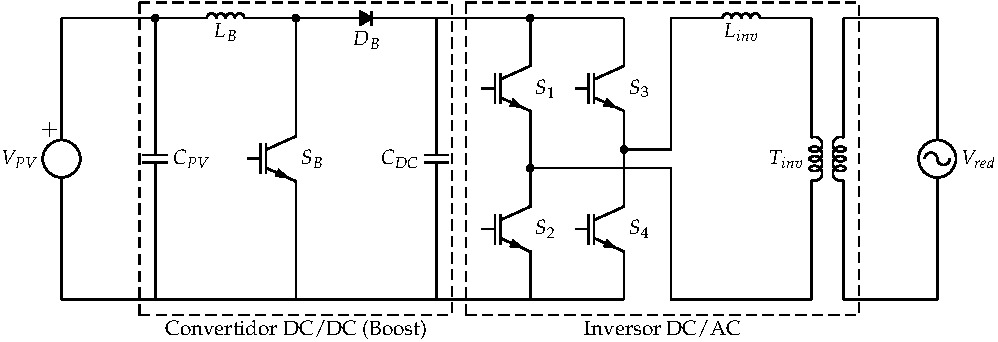
\includegraphics[scale=0.6]{../Figuras/InversorPV}
    \par\end{center}
  \begin{itemize}
  \item \textbf{Puente inversor}:\emph{ }realiza el troceado de la
    señal continua para convertirla en alterna
  \item \textbf{Filtro de salida}: elimina o atenúa los armónicos no
    deseados
  \item \textbf{Transformador}: adecua el valor de tensión de salida
    del puente al de la red y proporciona aislamiento galvánico entre
    la parte DC y AC\emph{. }
  \end{itemize}

\end{frame}
\begin{frame}[plain]
  \frametitle{Composición}

  \begin{center}
    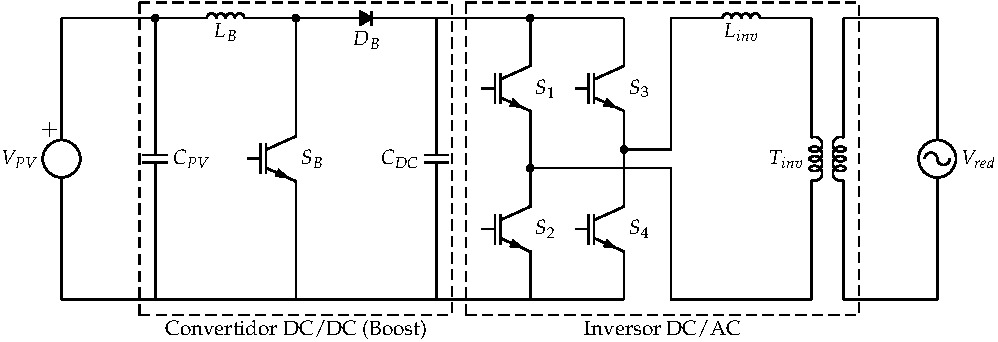
\includegraphics[scale=0.6]{../Figuras/InversorPV}
    \par\end{center}
  \begin{itemize}
  \item \textbf{Control}: realiza la supervisión de la entrada y
    salida del convertidor DC/DC y del puente inversor y entrega las
    consignas correspondientes para localizar y seguir el MPP del
    generador, y para obtener una señal sinusoidal con bajo contenido
    en armónicos en la salida del inversor.
  \end{itemize}

\end{frame}
\begin{frame}[plain]
  \frametitle{Funcionamiento: modulación SPWM}

  \begin{center}
    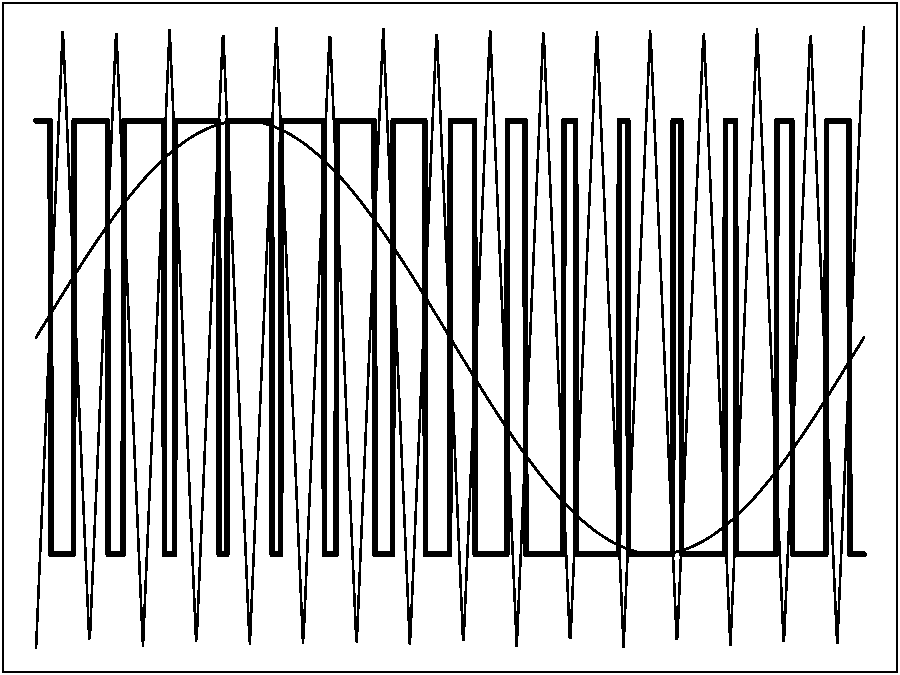
\includegraphics[scale=0.6]{../Figuras/SPWMMonofasico}
    \par\end{center}


\end{frame}
\begin{frame}
  \frametitle{Busqueda del Punto de Máxima Potencia}
  \begin{columns}[c]%{}


    \column{6cm}

    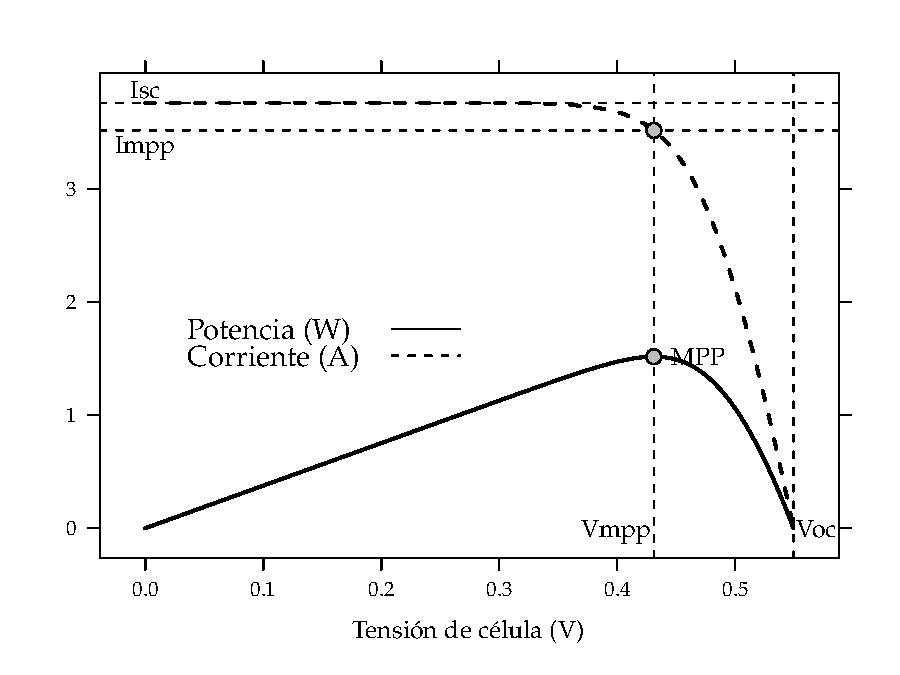
\includegraphics[scale=0.45]{../Figuras/CurvaIV_Ta20_G800}


    \column{6cm}

    \[
    \begin{cases}
      \frac{dP}{dV}>0 & 0<V<V_{mpp}\\
      \frac{dP}{dV}=0 & V=V_{mpp}\\
      \frac{dP}{dV}<0 & V_{mpp}<V<V_{oc}\end{cases}\]


  \end{columns}%{}

\end{frame}
\begin{frame}
  \frametitle{Busqueda del Punto de Máxima Potencia}
  \begin{columns}[c]%{}


    \column{6cm}

    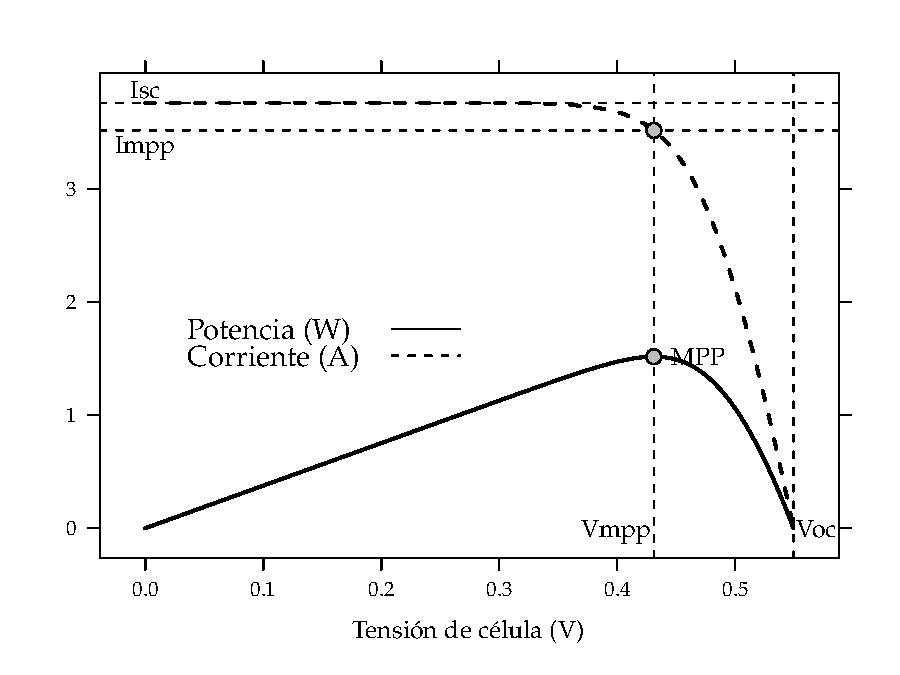
\includegraphics[scale=0.45]{../Figuras/CurvaIV_Ta20_G800}


    \column{6cm}

    \[
    \begin{cases}
      \frac{dI}{dV}>-\frac{I}{V} & 0<V<V_{mpp}\\
      \frac{dI}{dV}=-\frac{I}{V} & V=V_{mpp}\\
      \frac{dI}{dV}<-\frac{I}{V} & V_{mpp}<V<V_{oc}\end{cases}\]


  \end{columns}%{}

\end{frame}
\begin{frame}[plain]
  \frametitle{Uso del transformador}

  \begin{center}
    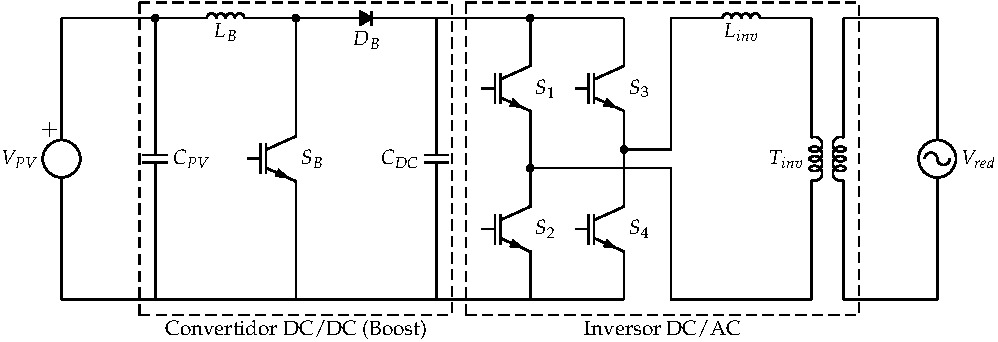
\includegraphics[scale=0.6]{../Figuras/InversorPV}
    \par\end{center}
  \begin{itemize}
  \item El transformador permite adecuar el nivel de tensión de salida
    del puente de conmutación a la tensión de red.
  \item La componente inductiva del transformador es parte del filtro
    de salida y sirve como acoplamiento entre la red eléctrica y la
    salida del inversor.
  \item Establece el aislamiento galvánico entre la entrada del
    inversor (DC) y la salida (AC).
  \end{itemize}

\end{frame}
\begin{frame}
  \frametitle{Uso del transformador}
  \begin{block} {Opciones comerciales}

    Existen tres opciones en el mercado de inversores de conexión a
    red:
    \begin{itemize}
    \item Inversores con transformador de salida en baja frecuencia
    \item Inversores sin transformador
    \item Inversores con transformador de alta frecuencia
    \end{itemize}
  \end{block}

\end{frame}

\begin{frame}
  \frametitle{Uso del transformador}
  \begin{block} {Normativa}

    La normativa vigente en España obliga al uso de un transformador
    de aislamiento o elemento equivalente para cumplir tres objetivos:
    \begin{enumerate}
    \item Aislar la instalación generadora para evitar la
      transferencia de defectos entre la red y la instalación
    \item Proporcionar seguridad personal
    \item Evitar la inyección de corriente continua en la red.
    \end{enumerate}

  \end{block}

\end{frame}

\begin{frame}
  \frametitle{Uso del transformador}
  \begin{block} {Nota de Interpretación Tecnica}
    \begin{itemize}
    \item Objetivos 1 y 2 se consiguen mediante la adecuada conexión
      de masas y tierras en el sistema.
    \item Objetivo 3: ``\textbf{la corriente continua inyectada en la red de
      distribución por una instalación generadora no será superior al
      0,5\% de la corriente nominal de la misma}'', cumplido ``\textbf{cuando
      se disponga en la instalación de un transformador separador
      entre el inversor y el punto de conexión de la red de
      distribución}''. \emph{Los inversores con transformador de alta
      frecuencia o sin transformador deben demostrar el cumplimiento
      de este requisito mediante un ensayo descrito en esta nota}.
    \end{itemize}

  \end{block}

\end{frame}

\begin{frame}
  \frametitle{'Islanding'}

  \begin{center}
    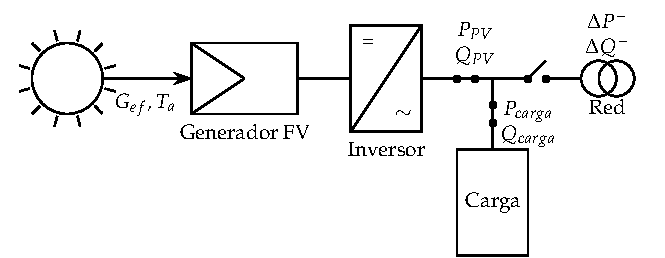
\includegraphics{../Figuras/Isla}
    \par\end{center}


\end{frame}
\begin{frame}
  \frametitle{'Islanding'}

  Antes de la desconexión:\[ \Delta P=P_{carga}-P_{PV}\]


\[
\Delta Q=Q_{carga}-Q_{PV}\simeq Q_{carga}\]


siendo:

\[
P_{carga}=\frac{V^{2}}{R_{carga}}\]


\[
Q_{carga}=\frac{V^{2}}{\omega L}-V^{2}\omega C\]



\end{frame}
\begin{frame}
  \frametitle{'Islanding'}
  \begin{itemize}
  \item $\Delta P^{-}>0\rightarrow P_{carga}>P_{PV}$. Al producirse la
    desconexión, dado que $P_{PV}$ no cambia, disminuye la potencia
    entregada a la carga, y por tanto baja la tensión.
  \item $\Delta P^{-}<0\rightarrow P_{carga}<P_{PV}$. Al producirse la
    desconexión, aumenta la potencia entregada a la carga, y por tanto
    sube la tensión.
  \item $\Delta Q^{-}>0\rightarrow Q_{carga}>0$. La carga es
    inductiva. Al producirse la desconexión, dado que el generador FV
    no entrega reactiva, la reactiva debe tender a 0, y por tanto
    aumenta la frecuencia.
  \item $\Delta Q^{-}<0\rightarrow Q_{carga}<0$. La carga es
    capacitiva.  La reactiva debe tender a cero, y por tanto disminuye
    la frecuencia.
  \end{itemize}

\end{frame}
\begin{frame}
  \frametitle{'Islanding'}

  Cuando las condiciones de trabajo del generador y el consumo antes
  de la desconexión son muy cercanas, existe una ventana de
  no-detección.

  \begin{center}
    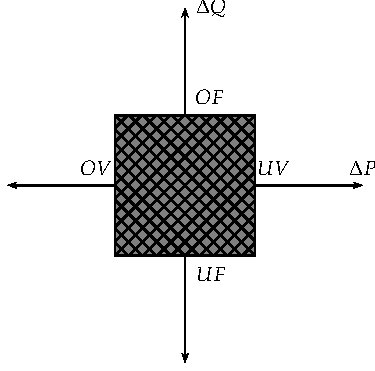
\includegraphics[scale=0.8]{../Figuras/NDZ}
    \par\end{center}


\end{frame}
\begin{frame}
  \frametitle{'Islanding'}
  \begin{block} {Estudio experimental IEA-PVPS}
    \begin{itemize}
    \item La probabilidad de que se de una situación de balance entre
      consumo y generación en una red de Baja Tensión está entre
      $\num{1e-5}$ y $\num{1e-6}$.
    \item Para que se de una situación de isla, este balance debe
      coincidir con una desconexión de la red: la probabilidad de
      ocurrencia simultánea de estos dos sucesos es virtualmente nula.
    \end{itemize}
  \end{block}

\end{frame}
\begin{frame}
  \frametitle{'Islanding'}
  \begin{block} {Estudio experimental IEA-PVPS}
    \begin{itemize}
    \item El riesgo eléctrico existente en cualquier red eléctrica es
      del orden de $\num{1e-6}$.
    \item Este estudio mostró que el riesgo de accidente eléctrico
      asociado a un sistema fotovoltaico funcionando en isla bajo los
      escenarios de mayor penetración fotovoltaica era inferior a
      $\num{1e-9}$.
    \item Este resultado indica que el riesgo asociado al accidente
      eléctrico por \textquotedblleft{}isla FV\textquotedblright{} no
      incrementa el riesgo que ya existe en las instalaciones
      eléctricas.
    \end{itemize}
  \end{block}

\end{frame}

\end{document}
